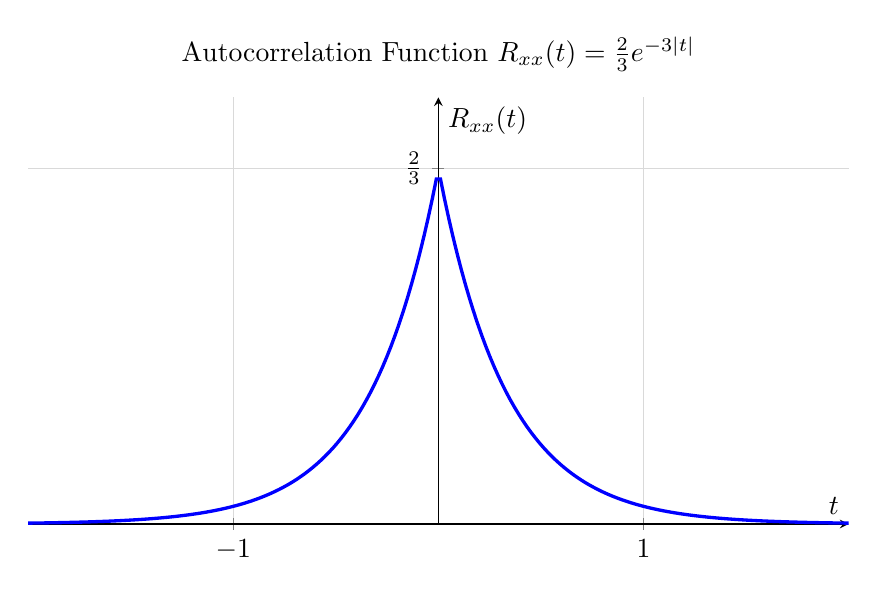
\begin{tikzpicture}
	\begin{axis}[
		width=12cm,
		height=7cm,
		title={Autocorrelation Function $R_{xx}(t) = \frac{2}{3}e^{-3|t|}$},
		xlabel={$t$},
		ylabel={$R_{xx}(t)$},
		axis lines=middle,
		xmin=-2, xmax=2,
		ymin=0, ymax=0.8,
		xtick={-1, 1},
		ytick={0.667},
		yticklabels={$\frac{2}{3}$},
		grid=major,
		grid style={line width=.1pt, draw=gray!30},
		]
		\addplot[blue, very thick, domain=-2:2, samples=200, no marks] {(2/3)*exp(-3*abs(x))};
	\end{axis}
\end{tikzpicture}